\part{Review of expansion loops in the energy sector}
\section{Industrial applications of expansion loops}
Thermal expansion and contraction is an everpresent issue for all piping systems. Thermal expansion is a natural phenomenon, linked with the kinetic energy of the moleculues. As the kinetic energy of moleculus increases, the intermolecular distance also increases. At macroscopic scales, this manifests as a potentially significant change in the shape, size, density, and volume of an object. Within the scope of a piping system, a change in temperature of a pipe fixed with supports is problematic because the change in shape will result in induced stress. Over time, these stresses may fatigue the piping system, causing leaks. A pipe may change temperature due to environmental effects (day-night cycle, sun shining on a pipe) or due to the working fluid working within the pipe (superheated steam, liquid nitrogen). Hence, building piping systems with the ability to combat this thermal expansion is important to protect the system. 

A few solutions exist to combat thermal expansion. One such example is the expansion loop. Figure \ref{expLoop} shows an expansion loop in a 2D and 3D configuration. The expansion loop acts to absorb the thermal expansion from the adjacent piping. The size and location of an expansion loop is primarily determined through code - for piping this is ASME B31.8. Before we can start designing a system, some requirements of the system must be first understood. Typically, one will know the working fluid of the system and hence can determine the temperature changes within the system. One will also most likely know where the working fluid is to go with flow rate requirements. This will determine the size and material of piping in the system. Equation \eqref{tempChange} shows how thermal expansion or contraction can be calculated for a given material.
\begin{equation}\label{tempChange}
    \Delta L = \alpha L_{pipe} \Delta T 
\end{equation}
where $\Delta L$ is the change in length, $\alpha$ is the coefficient of thermal expansion of the material, $L_{pipe}$ is the length of the pipe and $\Delta T$ is the change in temperature. Different materials will have different thermal properties and hence will expand or contract at different rates. However, these materials will also have different mechanical properties such as higher (or lower) working stress or modulus of elasticity. The pipe's thickness and outer diameter will also determine the maximum stress of the pipe. Figure \ref{themExpan} shows the rate at which different materials change length with temperature. It can be seen that plastic based materials expand much more quickly than metals in general. 
\begin{figure}[H]
    \centering
    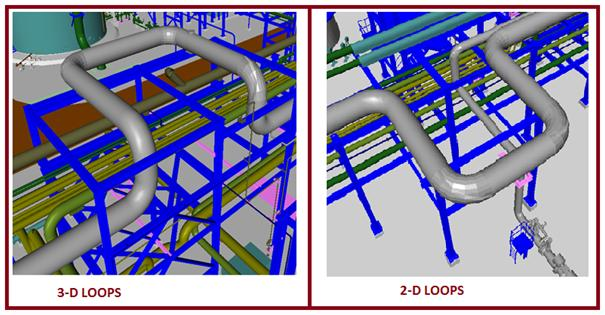
\includegraphics[width = 0.7\textwidth]{img/fig24.jpg}
    \caption{Expansion loops shown in a 2D and 3D configuration \cite{2d3d}.}
    \label{expLoop}
\end{figure}
\begin{figure}[H]
    \centering
    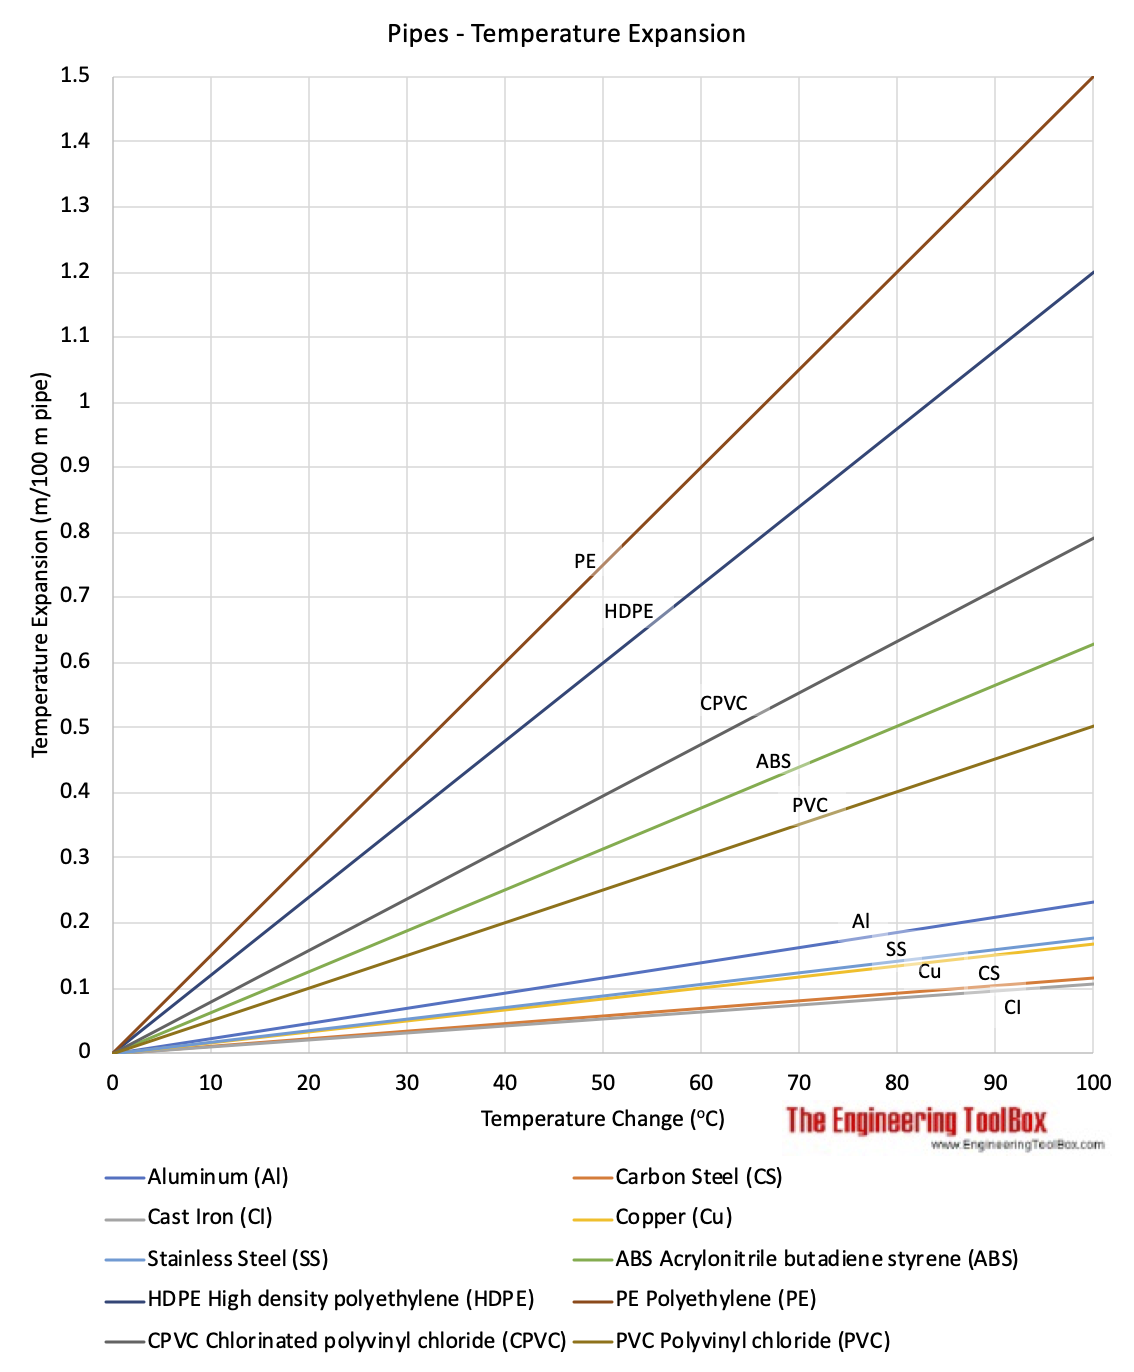
\includegraphics[width = 0.5\textwidth]{img/fig25.png}
    \caption{Thermal expansion for different materials \cite{therm}.}
    \label{themExpan}
\end{figure}
%\section{Design guidance for expansion loops}
%\section{Support systems for expansion loops}
\bibliographystyle{unsrtnat}
\bibliography{RefsA.bib}